\chapter{Metodologia}
\label{chap_metodologia}

A implementação foi realizada em Python, com uso das bibliotecas \texttt{numpy}, \texttt{matplotlib} e \texttt{PySimpleGUI}. O fluxo computacional foi organizado em funções para conversão de regra, evolução temporal, definição de condições iniciais e geração de visualizações.

No desenvolvimento prático desta entrega, as simulações utilizadas no relatório foram executadas pela interface gráfica empacotada em executável, sem uso de notebook \texttt{.ipynb}.

Foi construído um executável da interface gráfica utilizando \texttt{PyInstaller} \cite{pyinstaller}, atendendo ao requisito de entrega em formato executável. Na interface, o usuário informa os parâmetros da simulação e visualiza imediatamente a evolução espaço-temporal.

\begin{figure}[H]
    \centering
    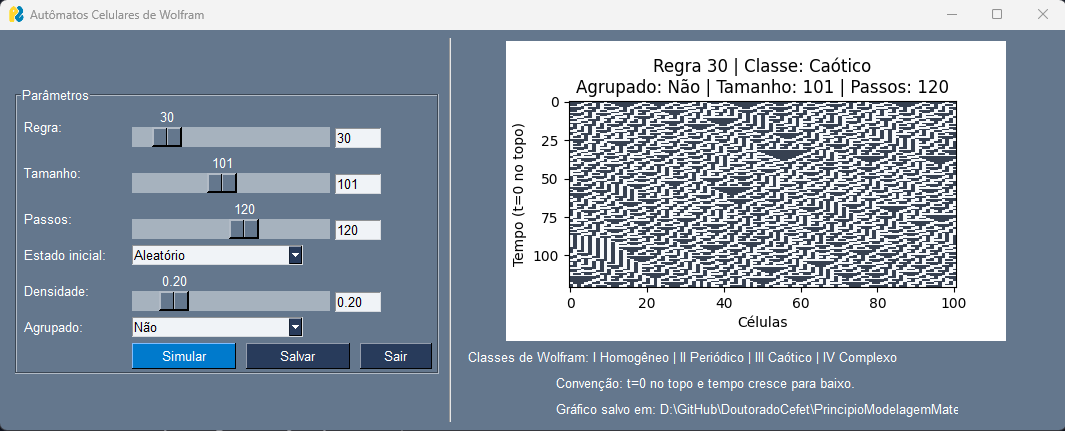
\includegraphics[width=0.78\textwidth]{figuras/imagem_executavel.png}
    \caption{Tela do executável desenvolvido para simulação dos autômatos celulares de Wolfram.}
    \label{fig:executavel-gui}
\end{figure}

O procedimento experimental adotado foi:
\begin{enumerate}
    \item converter o número da regra (0 a 255) para representação binária com 8 bits;
    \item aplicar a regra sobre vizinhança \((esquerda, centro, direita)\), com borda periódica;
    \item definir o estado inicial como central ou aleatório;
    \item configurar densidade inicial e opção de agrupamento dos sítios ativos;
    \item simular a evolução por um número fixo de passos;
    \item salvar a visualização espaço-temporal em formato PNG.
\end{enumerate}

Para garantir comparabilidade entre os cenários, os experimentos foram organizados em dois grupos:
\begin{itemize}
    \item classificação por classes de Wolfram, com \(tamanho=101\), \(passos=120\), estado inicial central, densidade \(0{,}5\) e sem agrupamento;
    \item seleção de duas regras por classe: homogênea (0, 255), periódica (4, 108), caótica (30, 90) e complexa (54, 110).
\end{itemize}

Como extensão da análise, também foram executadas variações com estado inicial aleatório, diferentes densidades e, em um subconjunto, ativação do parâmetro de agrupamento, permitindo discutir a sensibilidade dos padrões às condições iniciais.

